\documentclass[notes,11pt, aspectratio=169]{beamer}

\usepackage{pgfpages}

\usepackage{helvet}
\usepackage[default]{lato}
\usepackage{array}
\usepackage{tikz}
\usepackage{verbatim}
\usepackage{stackengine}
\setbeamertemplate{note page}{\pagecolor{yellow!5}\insertnote}
\usetikzlibrary{positioning}
\usetikzlibrary{decorations}
\usetikzlibrary{calc}
\usetikzlibrary{arrows}
\usetikzlibrary{decorations.markings}
\usetikzlibrary{shapes.misc}
\usetikzlibrary{matrix,shapes,arrows,fit,tikzmark}
\usepackage{amsmath}
\usepackage{mathpazo}
\usepackage{hyperref}
\usepackage{lipsum}
\usepackage{multimedia}
\usepackage{graphicx}
\usepackage{multirow}
\usepackage{graphicx}
\usepackage{dcolumn}
\usepackage{bbm}
\usepackage{appendixnumberbeamer}
\newcolumntype{d}[0]{D{.}{.}{5}}

\graphicspath{ {./figures/} }

\usepackage{changepage}
\usepackage{appendixnumberbeamer}



\usepackage{graphicx}
\usepackage[space]{grffile}
\usepackage{booktabs}

% These are my colors -- there are many like them, but these ones are mine.
\definecolor{blue}{RGB}{0,114,178}
\definecolor{red}{RGB}{213,94,0}
\definecolor{yellow}{RGB}{240,228,66}
\definecolor{green}{RGB}{0,158,115}

\hypersetup{
  colorlinks=true,
  linkbordercolor = {white},
  linkcolor = {blue},
  urlcolor= {blue}
}


%% I use a beige off white for my background
\definecolor{MyBackground}{RGB}{255,253,218}

%% Uncomment this if you want to change the background color to something else
%\setbeamercolor{background canvas}{bg=MyBackground}

%% Change the bg color to adjust your transition slide background color!
\newenvironment{transitionframe}{
  \setbeamercolor{background canvas}{bg=yellow}
  \begin{frame}}{
    \end{frame}
}

\DeclareMathOperator*{\argmin}{arg\,min} 
\DeclareMathOperator*{\Var}{var}

\setbeamercolor{frametitle}{fg=blue}
\setbeamercolor{title}{fg=black}
\setbeamertemplate{footline}[frame number]
\setbeamertemplate{navigation symbols}{} 
\setbeamertemplate{itemize items}{-}
\setbeamercolor{itemize item}{fg=blue}
\setbeamercolor{itemize subitem}{fg=blue}
\setbeamercolor{enumerate item}{fg=blue}
\setbeamercolor{enumerate subitem}{fg=blue}
\setbeamercolor{button}{bg=MyBackground,fg=blue,}



% If you like road maps, rather than having clutter at the top, have a roadmap show up at the end of each section 
% (and after your introduction)
% Uncomment this is if you want the roadmap!
\AtBeginSection[]
{
  \begin{frame}
   \frametitle{Today's Presentation}
      \tableofcontents[currentsection]
  \end{frame}
}
\setbeamercolor{section in toc}{fg=blue}
\setbeamercolor{subsection in toc}{fg=red}
\setbeamersize{text margin left=1em,text margin right=1em} 

\newenvironment{wideitemize}{\itemize\addtolength{\itemsep}{10pt}}{\enditemize}

\usepackage{environ}
\NewEnviron{videoframe}[1]{
  \begin{frame}
    \vspace{-8pt}
    \begin{columns}[onlytextwidth, T] % align columns
      \begin{column}{.58\textwidth}
        \begin{minipage}[t][\textheight][t]
          {\dimexpr\textwidth}
          \vspace{8pt}
          \hspace{4pt} {\Large \sc \textcolor{blue}{#1}}
          \vspace{8pt}
          
          \BODY
        \end{minipage}
      \end{column}%
      \hfill%
      \begin{column}{.42\textwidth}
        \colorbox{green!20}{\begin{minipage}[t][1.2\textheight][t]
            {\dimexpr\textwidth}
            Face goes here
          \end{minipage}}
      \end{column}%
    \end{columns}
  \end{frame}
}

\title[]{\textcolor{blue}{Open School Enrollment and Residential Sorting}}
\author[MCC]{}
\institute[Yale]{\small{\begin{tabular}{c}
Crossan Cooper  \\
Yale University \\
\end{tabular}}}

\date{\today}


\begin{document}

%%% TIKZ STUFF
\tikzset{   
        every picture/.style={remember picture,baseline},
        every node/.style={anchor=base,align=center,outer sep=1.5pt},
        every path/.style={thick},
        }
\newcommand\marktopleft[1]{%
    \tikz[overlay,remember picture] 
        \node (marker-#1-a) at (-.3em,.3em) {};%
}
\newcommand\markbottomright[2]{%
    \tikz[overlay,remember picture] 
        \node (marker-#1-b) at (0em,0em) {};%
}
\tikzstyle{every picture}+=[remember picture] 
\tikzstyle{mybox} =[draw=black, very thick, rectangle, inner sep=10pt, inner ysep=20pt]
\tikzstyle{fancytitle} =[draw=black,fill=red, text=white]
%%%% END TIKZ STUFF

% Title Slide
\begin{frame}
\maketitle
\end{frame}

\section{Introduction}

\begin{frame}{Overview}
\label{mapback}
  \begin{wideitemize}
    \item We know that where you live and where you go to school matter for both short- and long-run outcomes (Chetty et al. 2014, Altonji and Mansfield 2018)
    \item These two often go hand-in-hand in the US because of neighborhood-based school assignment, potentially exacerbating economic inequality
    \item In the last 30 years, \textit{various} school choice policies in the US have sought to improve \textcolor{red}{(a)} school quality, \textcolor{green}{(b)} access to high quality schools, or \textcolor{blue}{(c)} both
    \begin{wideitemize}
    \item Private (e.g. vouchers, tax credits, ESA's) and public (e.g. charter schools, magnet schools, open enrollment)
    \end{wideitemize}
    \item \textbf{This project?} Explore how intradistrict choice programs affect residential sorting within and across districts
    \begin{wideitemize}
    \item In the future, explore welfare consequences in a model where schools face competition and households can sort across neighborhoods
    \end{wideitemize}
  \end{wideitemize}
  \hyperlink{map}{\beamerbutton{Open Enrollment Map}}
\end{frame}



\begin{frame}{Literature}
\begin{wideitemize}
\item \textbf{Equilibrium residential sorting:} Tiebout 1956, Nechyba 2000, Epple and Romano 2003, Bayer et al. 2007, Ferreyra 2007, Avery and Pathak 2021
\item \textbf{Competitive effects of school choice:} Hoxby 2003, Rothstein 2006, MacLeod and Urquiola 2015, Barseghyan et al. 2019, Allende 2019, Neilson 2021, Campos and Kearns 2022
\begin{wideitemize}
    \item \textcolor{blue}{Hope to provide additional evidence for/against competitive effects of choice}
\end{wideitemize}
\item \textbf{Sorting responses to choice policies:} Reback 2005, Baum-Snow and Lutz 2011, Brunner et al. 2012, Altonji et al. 2015, Zheng 2022
\begin{wideitemize}
    \item \textcolor{blue}{No existing evidence on sorting responses to \textit{intradistrict} open enrollment}
\end{wideitemize}
\item \textit{Outside of the direct purview of this project:} Akbarpour et al. 2022
\end{wideitemize}
\end{frame}

\begin{frame}{This Project}
\begin{alertblock}{Research Question 1: Housing Prices}
  What happens to the distribution of home prices after the switch from neighborhood assignment to open enrollment?
\end{alertblock}
\begin{exampleblock}{Research Question 2: Location}
  Do families relocate because of the policy? If so, are there differences in relocation patterns by family race or wealth level?
\end{exampleblock}
\begin{block}{Research Question 3: Welfare}
  What happens to household welfare after the introduction of open enrollment policies?
  % Which mechanism out of residential sorting and competitive incentives to improve school quality is stronger in equilibrium?
\end{block}
\medskip 
\begin{wideitemize}
    \item No existing evidence on \textcolor{red}{(1)} and \textcolor{green}{(2)} for intra-district open enrollment policies. The sign and magnitude of welfare changes in \textcolor{blue}{(3)} depends on how households and schools respond to open enrollment
\end{wideitemize}
\end{frame}

\begin{frame}{Data}
\begin{wideitemize}
\item Today?
\begin{wideitemize}
\item \textbf{Aggregated Home Prices:} FHFA HPI, Zillow HVI
\item \textbf{Neighborhood Demographics:} ACS, Census
\item \textbf{School District Characteristics:} NCES CCD
\item \textbf{Open Enrollment Adoption Dates:} NAPCS
\end{wideitemize}
\item Future?
\begin{wideitemize}
  \item \textbf{Home Prices and Characteristics:} CoreLogic
  \item \textbf{School Attendance Zone Boundaries:} SABINS
\end{wideitemize}
\end{wideitemize}
\end{frame}

\section{A Toy Model}

\begin{frame}{Toy Model Inspired by Avery and Pathak (2021)}
\begin{wideitemize}
\item Consider a school district with two neighborhoods, one with a school of quality $q_1$ and one with a school of quality $q_2$
\item Households of type $x$ choose their neighborhood $n$ to solve \[V(x) = \max_{q_n \in \{q_1, q_2\}} [u(x, q_n) = x\cdot q_n - p(q_n)] \]
\item Home prices are competitive and depend only on the quality of the school, where \[q_n = E[x|x \in n]\]
\item A household will leave the district if their highest possible neighborhood utility does not exceed the highest utility $O(x)$ they can achieve from schools outside the district \[O(x) = \max_q [x\cdot q - p(q) - \textcolor{red}{C}] = \frac{x^2}{2} - \textcolor{red}{C}\]
where $\textcolor{red}{C}$ captures a household's moving cost

\end{wideitemize}
\end{frame}

\begin{frame}{Exiting the District}
\begin{wideitemize}
\item A household of type $x$ will exit the district whenever
\begin{equation*}
O(x) = \frac{x^2}{2} - \textcolor{red}{C}  >   x \cdot q_n - \frac{q_n^2}{2} = V(x)
\end{equation*}
\item This condition holds up iff
\begin{equation*}
 \frac{(x-q_n)^2}{2} > \textcolor{red}{C}
\end{equation*}
for either $n=1$ or $n=2$. Remember, higher $\textcolor{red}{C} = $ higher moving cost
\item \textbf{Intuition?} Household will pay the moving cost and exit the district if it can't find a school close enough to its \textit{ideal} level
\end{wideitemize}
\end{frame}

\begin{frame}{When will everyone stay under Neighborhood Assignment?}
\begin{figure}
\centering
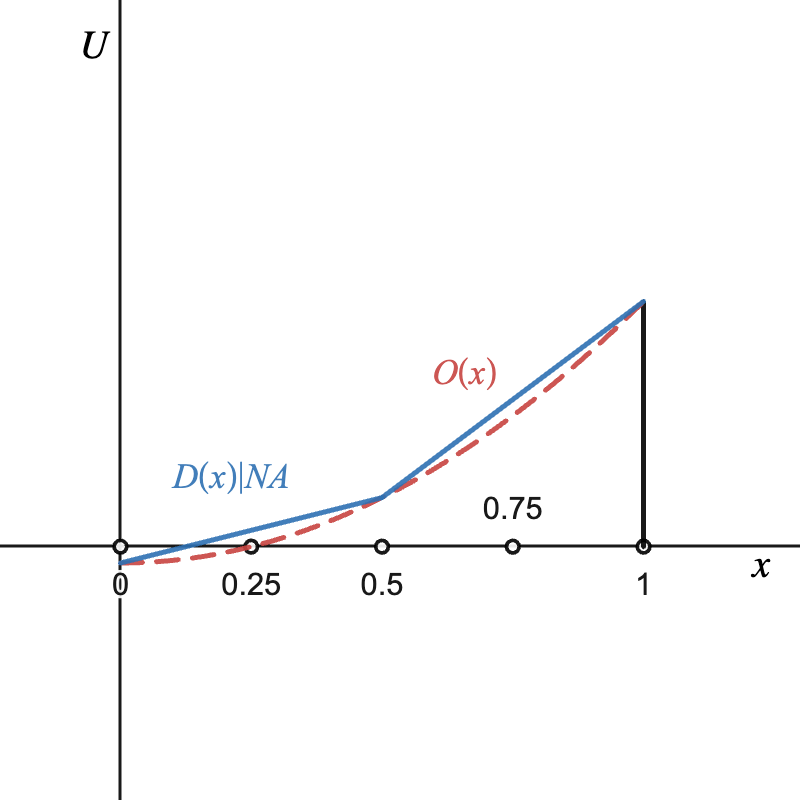
\includegraphics[width=0.65\textwidth]{figures/neighborhood.png}
\caption{Sorting Neighborhood Equilibrium with $x \sim U(0,1)$}
\end{figure}
\end{frame}

\begin{frame}{When will everyone stay under School Choice?}
\begin{figure}
\centering
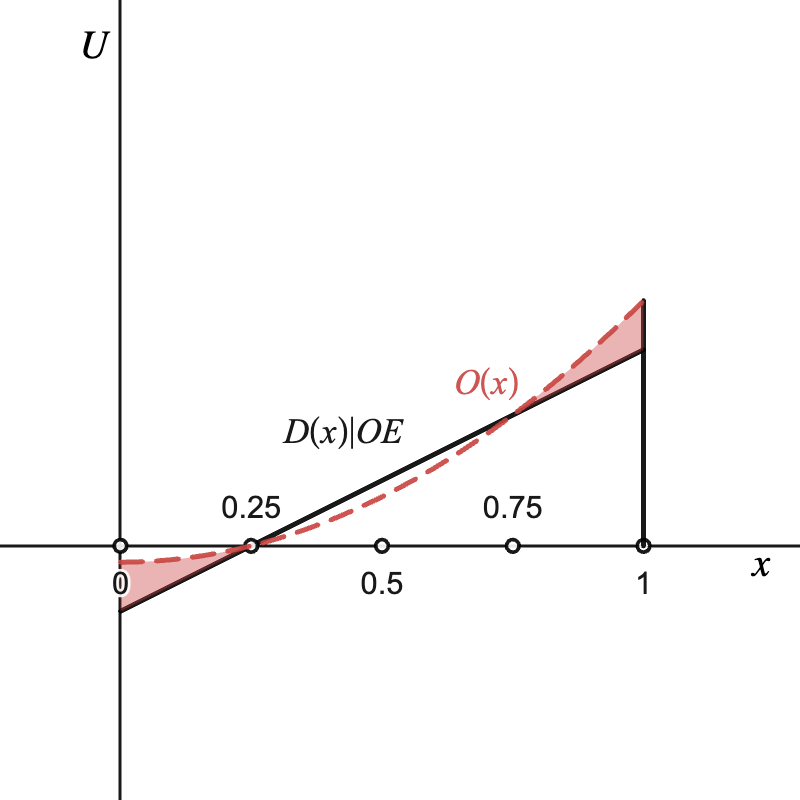
\includegraphics[width=0.75\textwidth]{figures/school_choice.png}
\caption{School Choice Equilibrium with $x \sim U(0,1)$}
\end{figure}
\end{frame}

\begin{frame}{Toy Model Insights}
\begin{wideitemize}
\item \textcolor{blue}{The key mechanism?} When school choice is introduced, school qualities equalize. Competitive housing market leads to
\begin{wideitemize}
\item $\textcolor{green}{\uparrow}$ home prices in neighborhood with originally lower-quality school
\item $\textcolor{green}{\downarrow}$ home prices in neighborhood with originally higher-quality school
\end{wideitemize}
\item Lots of reasons to think this pattern might not hold up in practice:
\begin{enumerate}
    \item Homes are differentiated by quality
    \item Schools do not adjust to the same quality under school choice because of exogenous fixed factors and frictions in the choice process
    \item Home prices are sticky and low-type families may be immobile in their residential choices
\end{enumerate} 
\end{wideitemize}
\end{frame}

\section{Empirical Results}

\begin{frame}{Adopters of Intradistrict Open Enrollment}
% summary statistics table
\begin{table}[h] \centering 
\renewcommand{\arraystretch}{1.25}
    %\caption{Student Summary Statistics} 
    \label{sumstats} 
  \scriptsize 
  \begin{tabular}{@{\extracolsep{5pt}}lcccccccc} 
  \\[-1.8ex]\hline 
  \hline \\[-1.8ex] 
  \textit{Districts} & Adoption & State & \# Schools & \# Students & \$/Student & STR & \% URM & \% FRPL \\ 
  \hline \\[-1.8ex] 
  Camden & 2016 & NJ & 20 & 7,638 & \$28,845 & 9.5 & 98.6\% & 51.3\% \\
  Denver & 2011 & CO & 206 & 92,039 & \$12,639 & 15.0 & 70.1\% & 55.9\% \\
  Grand Prairie & 2012 & TX & 41 & 29,200 & \$9,984 & 15.4 & 86.2\% & 67.5 \% \\
  Indianapolis & 2018 & IN & 59 & 26,410 & \$12,452 & 14.0 & 73.9\% & 63.9\% \\ 
  Newark & 2014 & NJ & 64 & 40,448 & \$20,566 & 14.5 & 91.1\% & 61.1 \% \\  
  Pinellas County & 2003 & FL & 157 & 100,948 & \$9,952 & 13.4 & 40.9\% & 44.7\% \\  
  Washington & 2014 & DC & 113 & 49,065 & \$22,406 & 12.1 & 81.5\% & -- \\  
  \midrule
  US Average & -- & -- & 5.4 & 2,859 & \$17,050 & 15.6 & 35.0\% & 39.7\% \\  
  \midrule \midrule
  \multicolumn{9}{l}{\parbox{15cm}{Note: STR denotes student-teacher ratio. Aside from adoption dates, all school district data is from the 2018-2019 NCES CCD, the last year in which district financial data is available. School districts reporting 0 enrollment and non-traditional districts (i.e. charters) are dropped from the sample when calculating national averages.}}
  \end{tabular}
  \end{table} 

\end{frame}

\begin{frame}{Home Price Responses to Intradistrict Open Enrollment}
\label{giniback}
\centering
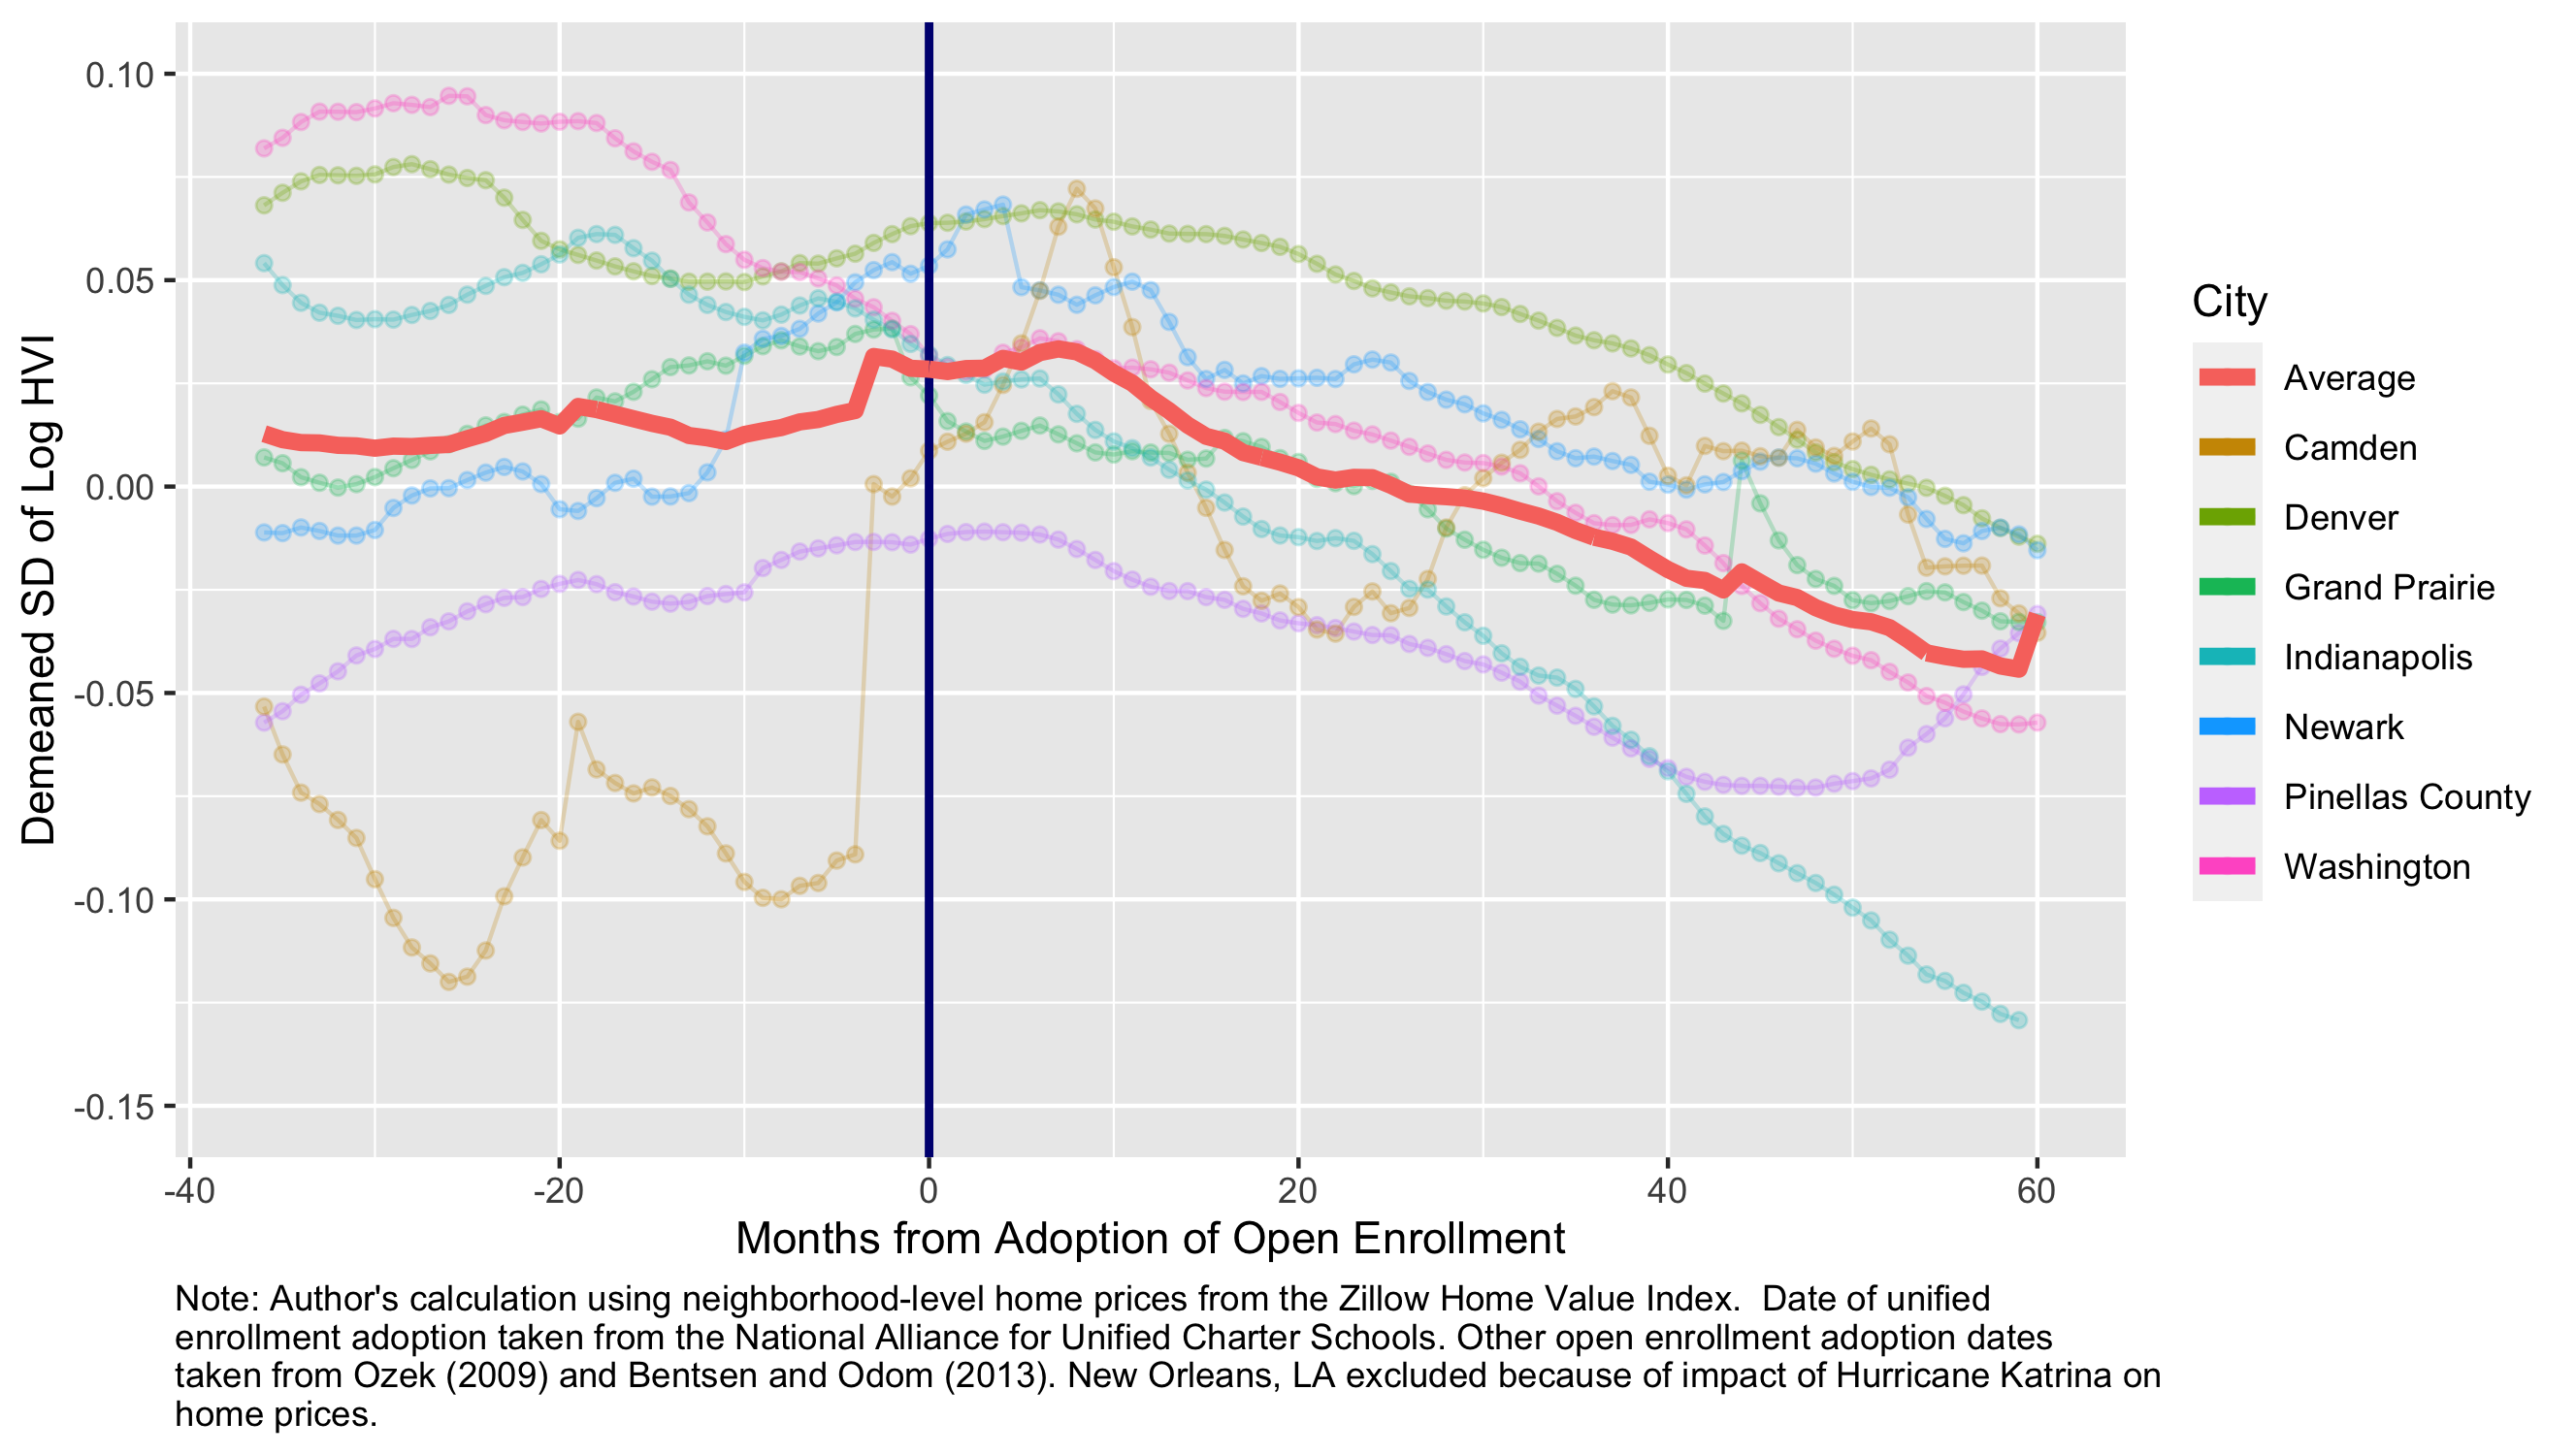
\includegraphics[width=0.9\textwidth]{figures/demeaned_hpi_sd_MONTHLY.png}
\hyperlink{gini}{\beamerbutton{Gini Index}}
\end{frame}

% \begin{frame}{School District Synthetic Controls Framework}
% % be explicit about treatment and control group
% \begin{wideitemize}
% \item Want to know how open enrollment impacts the distribution of home prices within a school district. But no clear control group
% \item \textbf{Potential solution?} Adopt augmented synthetic control method (Ben-Michael et al. 2021) to construct valid synthetic controls for treated districts and deal with staggered policy adoption
% \item \textit{Pool of potential control school districts:} 4418 districts in the top 25\% of student enrollment (above 2169 students)
% \item \textit{Matching strategy:} pre-treatment levels of \textcolor{blue}{(1)} outcome variable and \textcolor{blue}{(2)} per-student spending, \textcolor{blue}{(3)} student-teacher ratio, \textcolor{blue}{(4)} \% free and reduced price lunch, \textcolor{blue}{(5)} \% under-represented minority, \textcolor{blue}{(6)} number of schools, \textcolor{blue}{(7)} number of students
% % \item SE's are clustered at the district-year level
% % \item \textbf{Identifying Assumption:} without the open enrollment policy, the difference in district-level outcomes between observably similar districts is constant over time
% \end{wideitemize}
% \end{frame}

% \begin{frame}{School District Synthetic Controls Results}
% % figure of home price appreciation after the adoption date separately for high and low neighborhoods
% \end{frame}

\begin{frame}{Neighborhood Diff-in-Diff Framework}
% be explicit about treatment and control group
\begin{wideitemize}
\item Consider a staggered DiD design at the neighborhood-year level\[Y_{nt} = \alpha + \sum_{k \ne -1 } \textcolor{red}{\beta_k} \cdot \mathbf{1}\{\text{$k$ years from treatment}\}_{dt} + \mathbf{X}_{nt}' \Gamma + \phi_n + \gamma_t + \epsilon_{nt} \]
where $\mathbf{X}_{nt}$ is a vector of baseline neighborhood characteristics $\times$ year dummies
% need to think about where to cluster SE's
\item Treated neighborhoods are those in the bottom quintile of the housing price distribution, control neighborhoods are those in the top quintile
\item \textbf{Identifying Assumption:} without the open enrollment policy, the difference in neighborhood-level house appreciation / demographics across neighborhoods in the same school district is constant over time
\end{wideitemize}
\end{frame}

\begin{frame}{Neighborhood Diff-in-Diff: House Appreciation}
\begin{figure}
\centering
\includegraphics[width=0.8\textwidth]{figures/appreciation_did.png}
\caption{Top Quintile Neighborhoods vs. Bottom Quintile Neighborhoods}
\end{figure}
\end{frame}

% \begin{frame}{Neighborhood Diff-in-Diff: Median HH Income}

% \end{frame}

% \begin{frame}{Neighborhood Diff-in-Diff: Percent URM}

% \end{frame}

% \section{Descriptive Hedonics}

% \begin{frame}{Hedonics}
% \begin{wideitemize}
% \item Consider a hedonic model of neighborhood home prices %
% \[ \log p_{nt} = \textcolor{blue}{\beta_t} \mathbf{X}_{nt} + \epsilon_{nt} \] where %
% $\mathbf{X}_{nt}$ is a vector of neighborhood characteristics including neighborhood school quality, median household income, and average level of parental education
% \item What happens after a district moves from neighborhood assignment to open enrollment? In particular, how does $\textcolor{blue}{\beta_t^{school}}$ change? 
% \item Intuition from the school quality capitalization literature (e.g. Black 1999) suggests that $\textcolor{blue}{\beta_t^{school}}$ $\uparrow$ in catchment areas of low-performing schools and $\downarrow$ in catchment areas of high-performing schools
% \end{wideitemize}
% \end{frame}

% \begin{frame}{Hedonic Model Parameter Estimates}
% % make a table here
% \end{frame}

\section{Looking Ahead}

% \begin{frame}{Sketching a Model}
% \begin{wideitemize}
%     \item Want to adopt a sufficient statistics approach to estimate the equilibrium response to the school choice policy
% \end{wideitemize}
% \end{frame}

\begin{frame}{Conclusion}
\begin{wideitemize}
    \item \textbf{What did I show you today?}
    \begin{enumerate}
    \item A toy model highlighting two related mechanisms (i.e. \textcolor{red}{changes to home prices \& changes to school quality}) that might induce out-of-district migration after open enrollment
    \item Reduced-form evidence that neighborhood-level home prices and demographic characteristics have an anticipatory response to open enrollment policies
    \end{enumerate}
    \item \textbf{What is coming next?}
    \begin{enumerate}
    \item A richer model with vertical and horizontal differentiation to characterize sorting across neighborhoods and school districts
    \item Additional reduced-form work using CoreLogic and (hopefully) some individual-level data
    \item Robustness checks on existing results
    \end{enumerate}
\end{wideitemize}
\end{frame}


\begin{frame}
  \centering \Huge
  %\emph{Thank You For Coming!}
  Thank You For Coming!

  \bigskip 
  \centering \small
  Questions or comments? \url{crossan.cooper@yale.edu}
\end{frame}

\section*{Extra Slides}

\appendix

\begin{frame}{Landscape of Open Enrollment in the US} 
% insert the map here
\label{map}
\centering
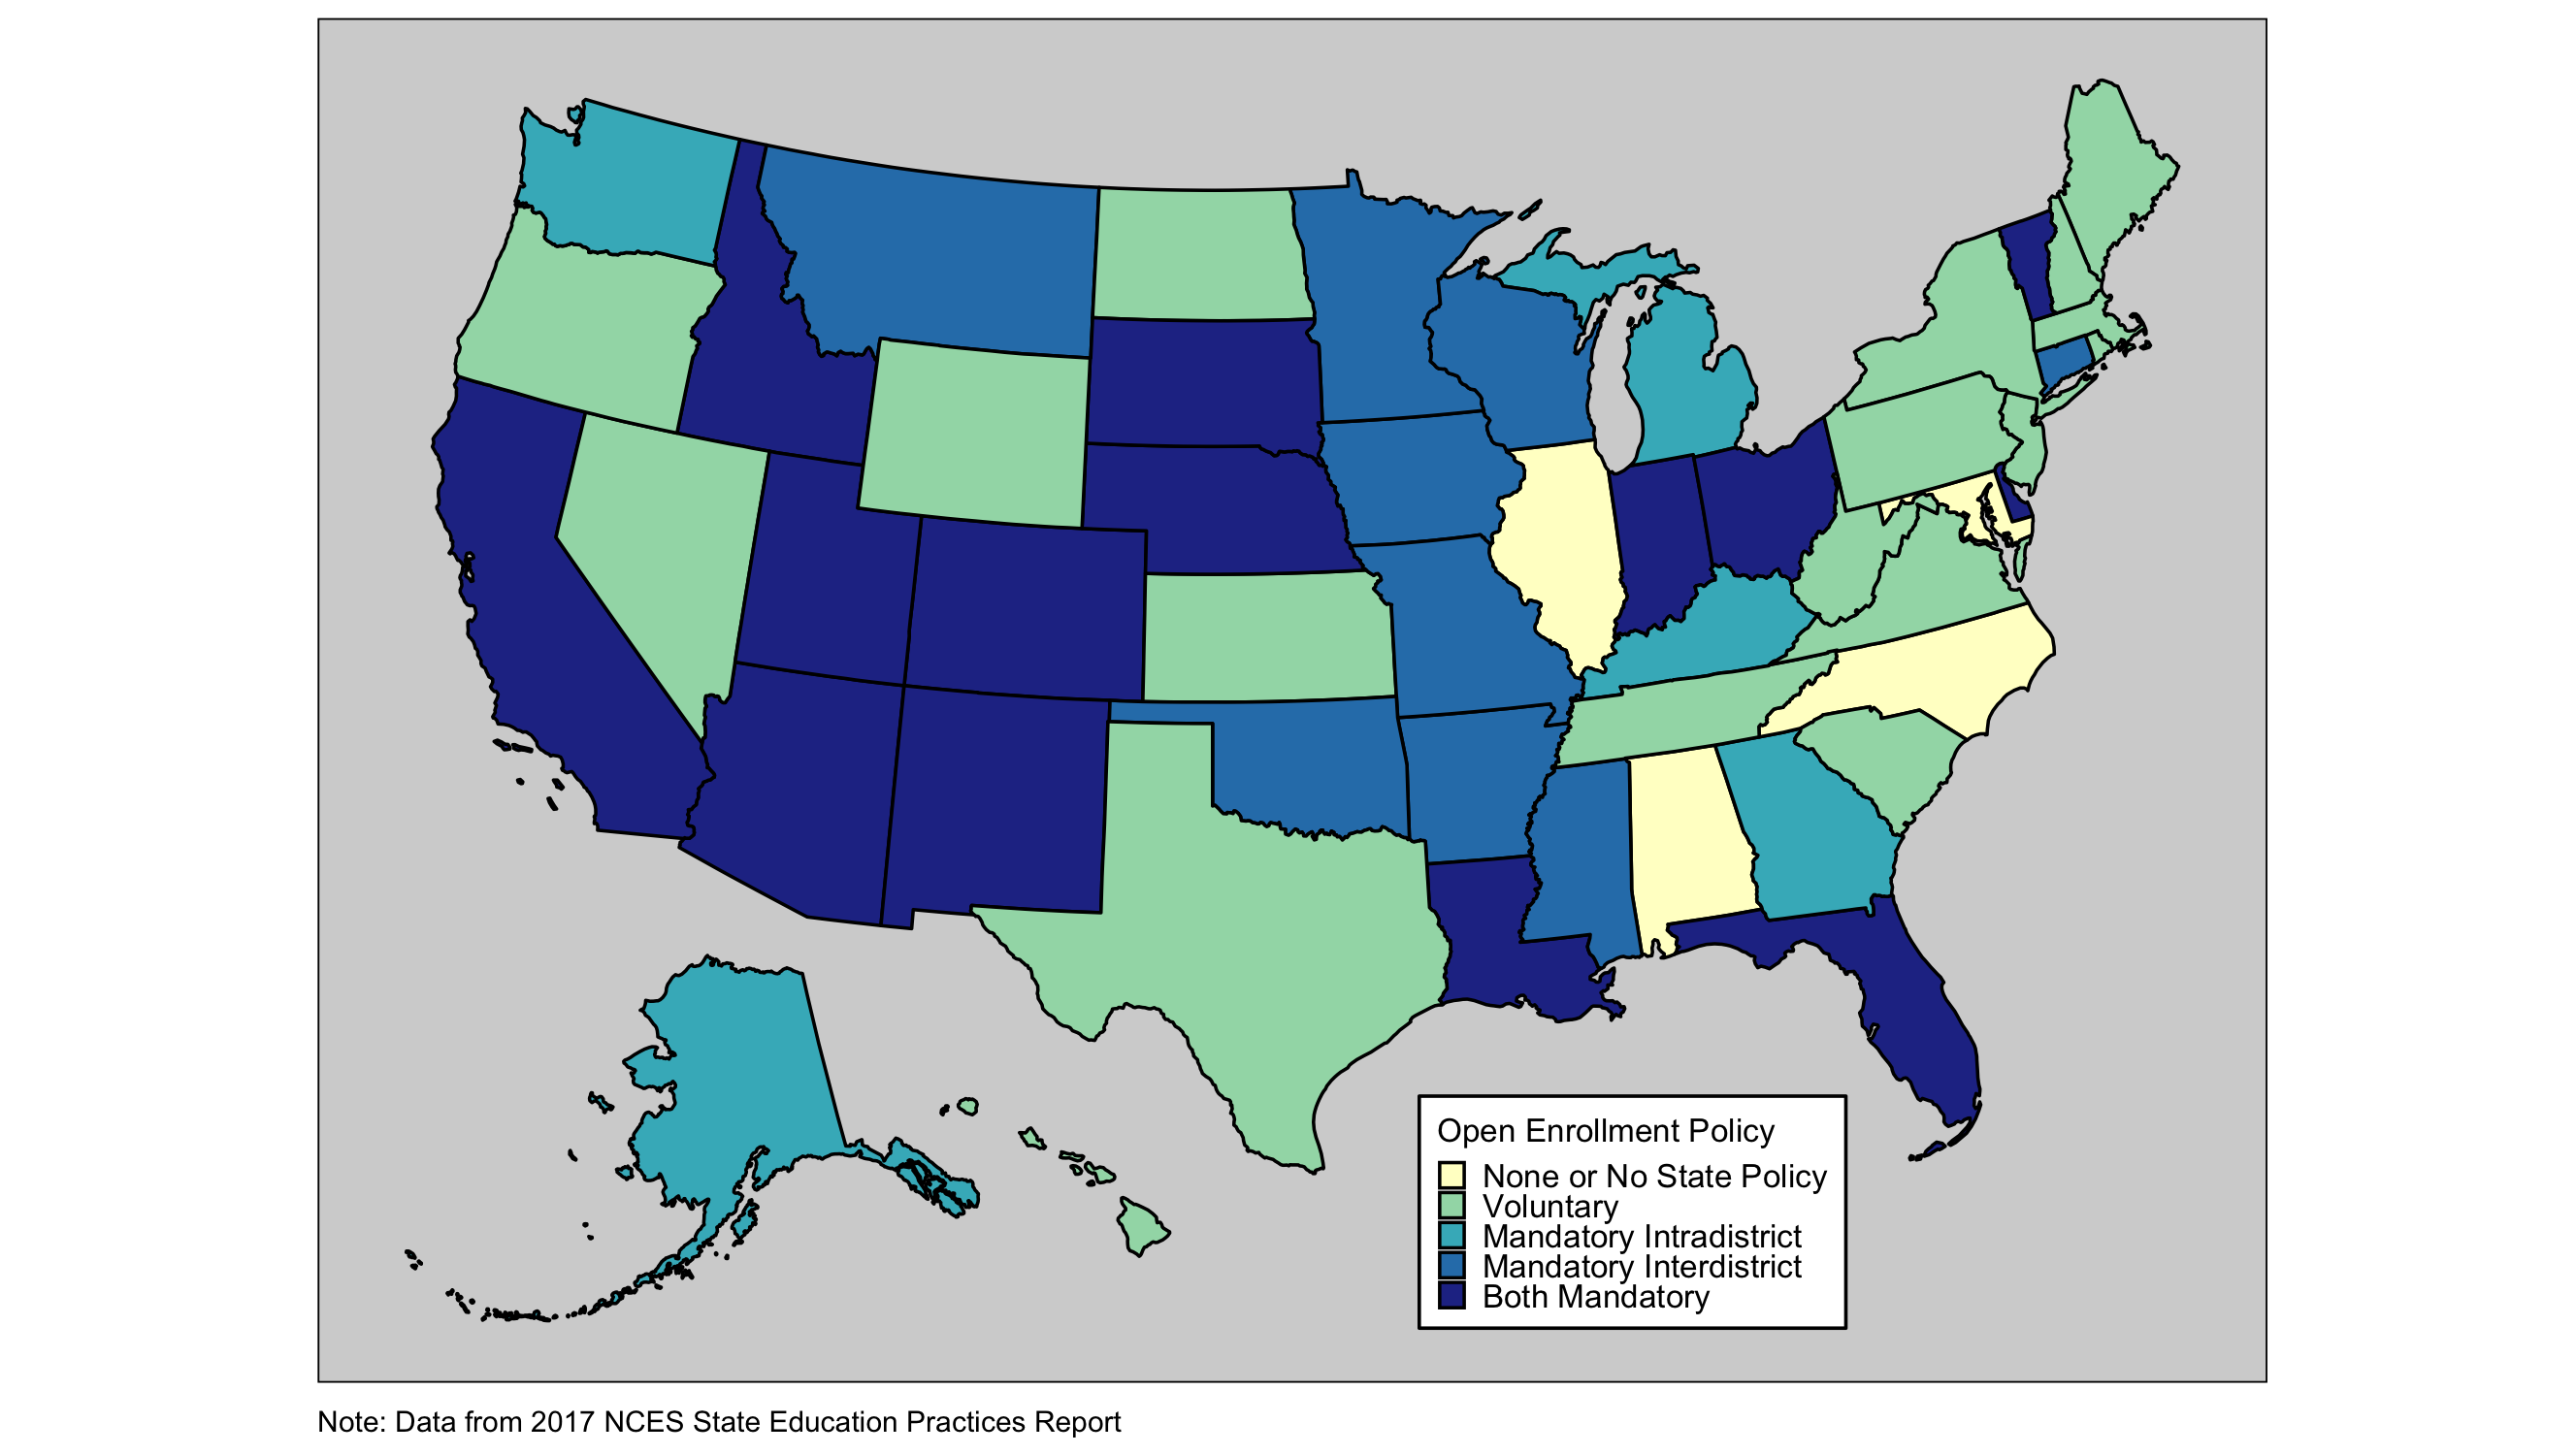
\includegraphics[width=0.8\textwidth]{figures/policies_map.png}
  \begin{wideitemize}
    \item Open enrollment plans began in the US in 1988 and are still being debated: Kansas just passed open enrollment legislation for the 2024-2025 school year \hyperlink{mapback}
    %\item Practitioners and policy-makers distinguish between \textcolor{red}{voluntary} and \textcolor{red}{mandatory} open enrollment as well as \textcolor{green}{intradistrict} versus \textcolor{green}{interdistrict} transfer policies
  \end{wideitemize}
\end{frame}

\begin{frame}{Home Price Responses to Intradistrict Open Enrollment}
\label{gini}
\centering
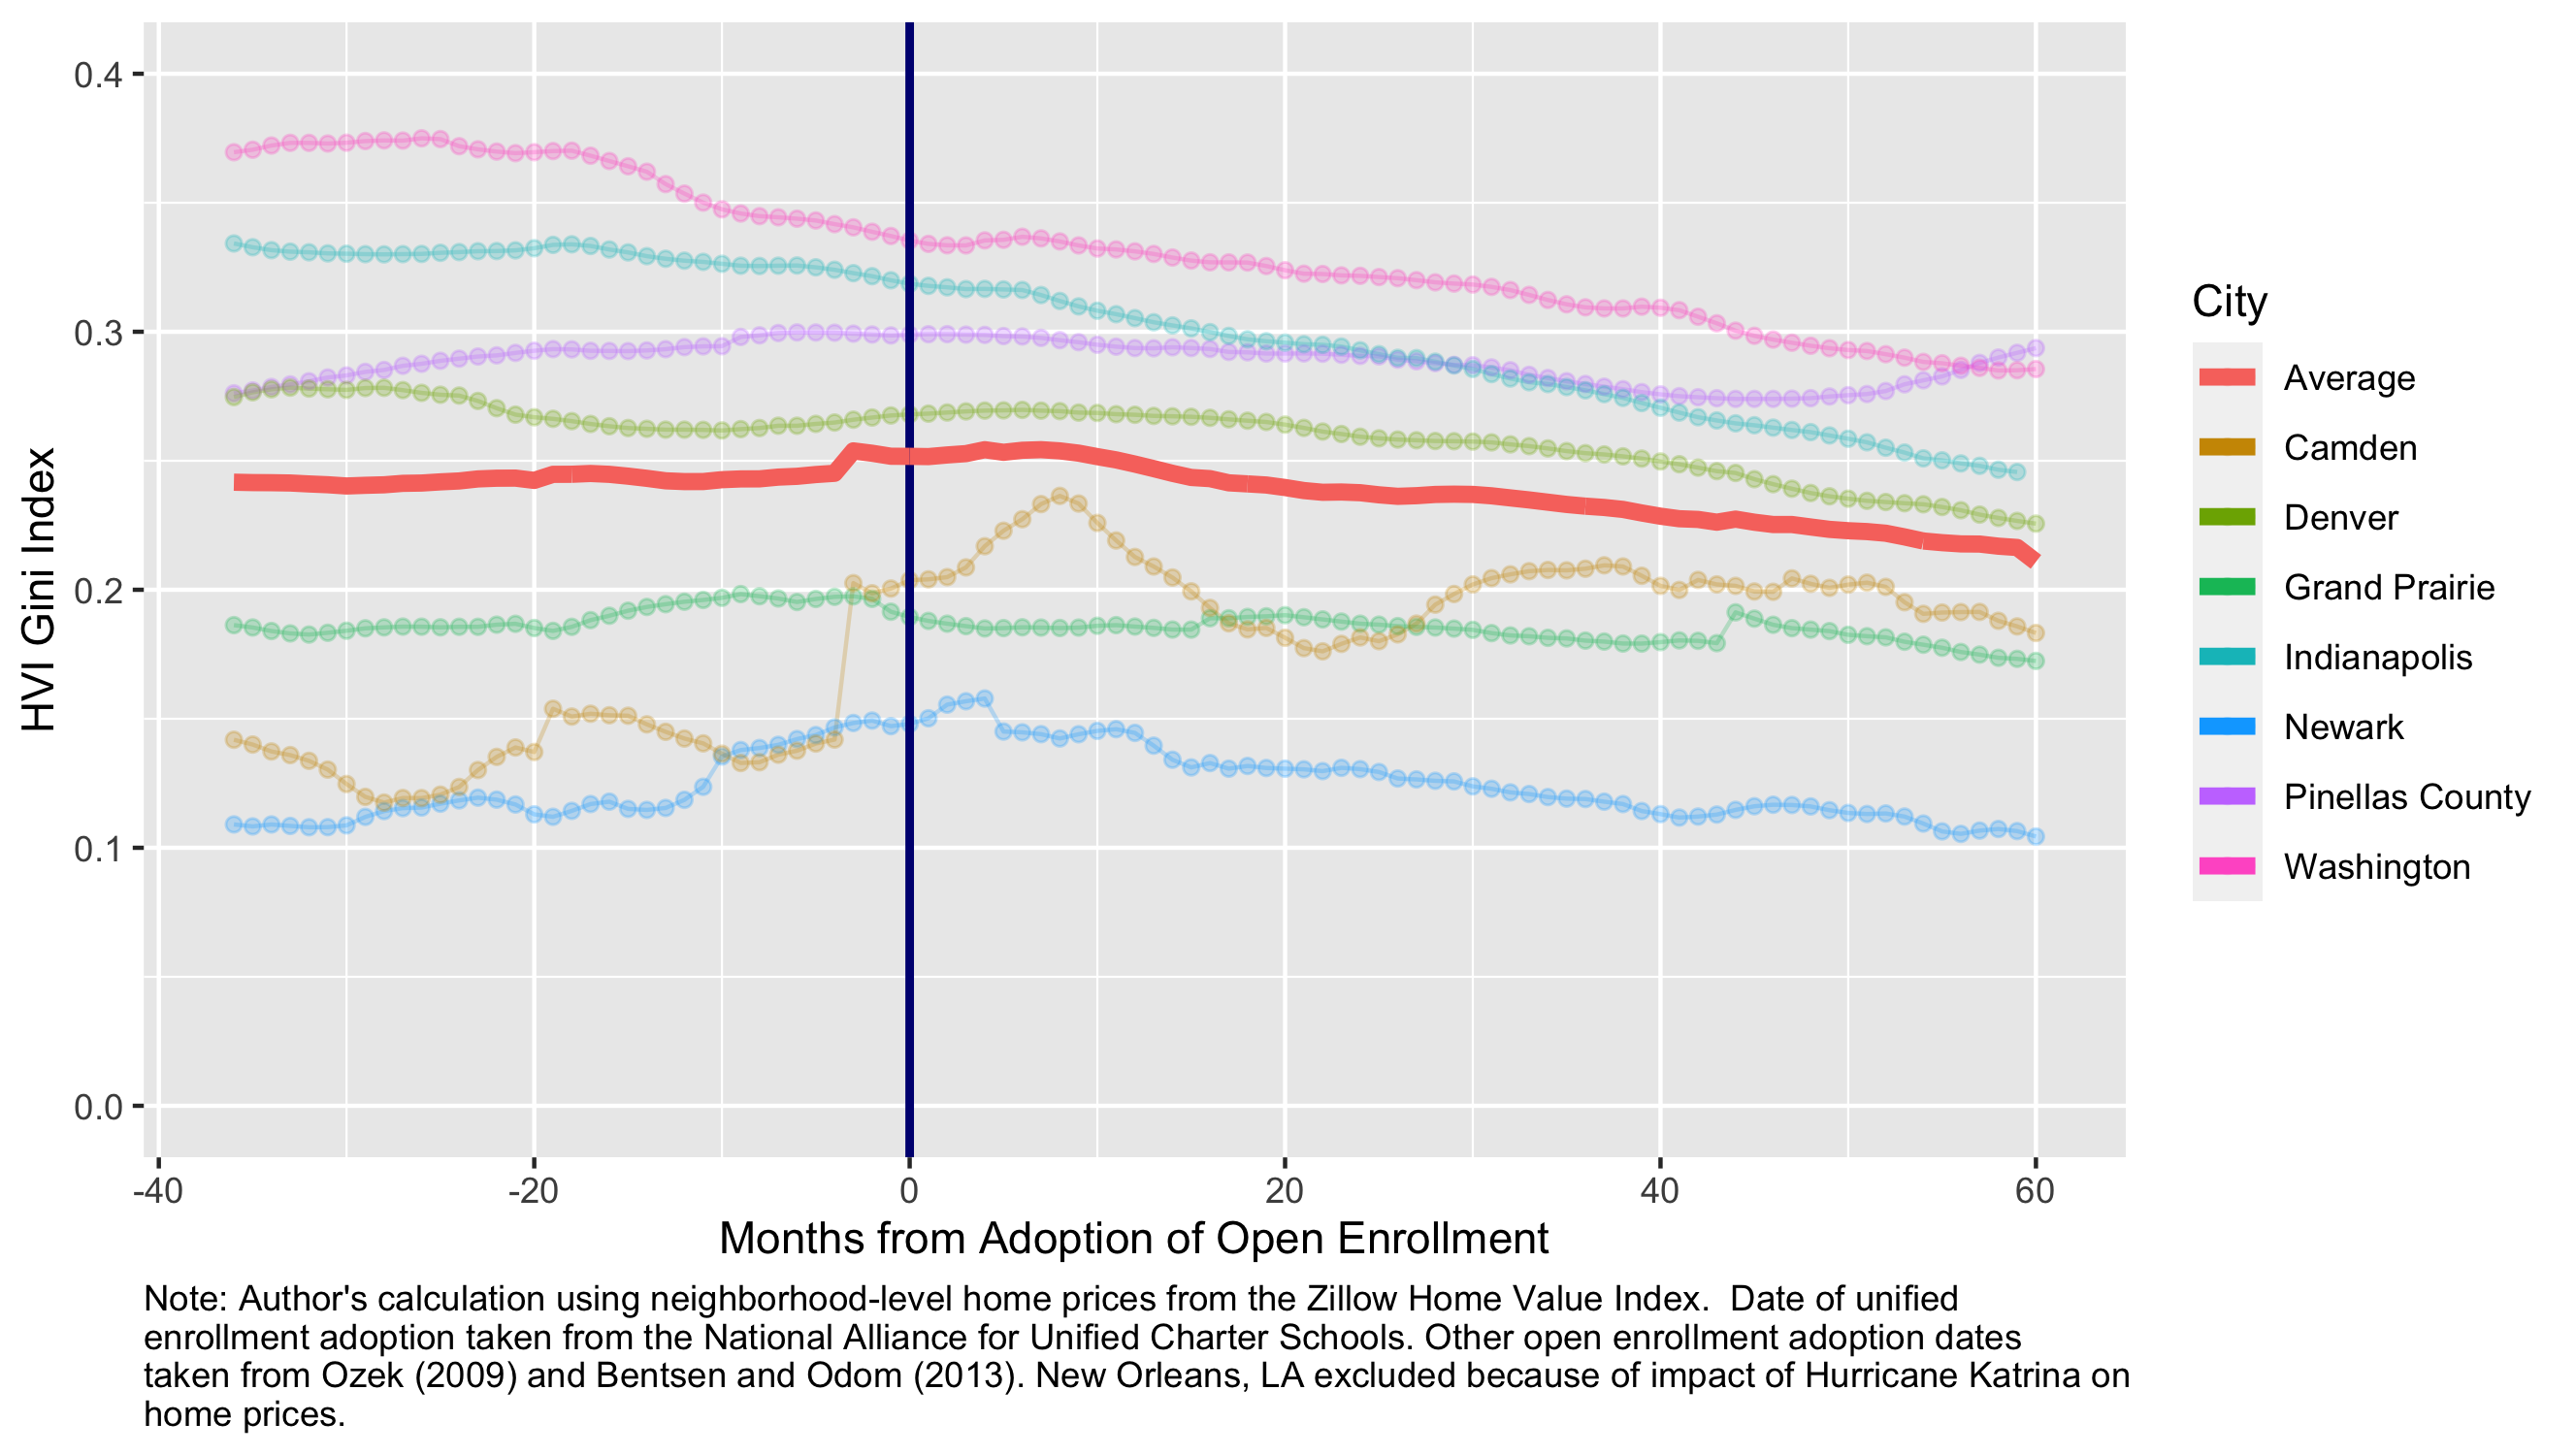
\includegraphics[width=0.9\textwidth]{figures/monthly_gini.png}
\hyperlink{giniback}{\beamerbutton{Back}}
\end{frame}


\end{document}